\chapter{Analyse und Performance}\label{kap7}
\section{Produktvergleich mit Anforderungsliste}\label{vergleich}
Um das Endresultat im Kontext der zuvor definierten Anforderungen analysieren zu können, wird sich auf die Anforderungsliste aus \autoref{kap1} berufen, welche aus Übersichtsgründen in \autoref{tab:Anforderungsliste2} noch einmal abgebildet ist.\\ 
Im Rahmen der Arbeit wurde eine zuvor eingerichtete \textbf{CAN-Schnittstelle} zum Senden von CAN-Nachrichten genutzt. Dazu werden die Signale in die nach \autoref{CANNachrichten} definierten Befehle unterschieden, sodass sich eine sinnvolle und benutzerfreundliche Menge an übermittelbaren Nachrichten ergibt. Es ist sowohl möglich die benötigten Schaltbefehle zu übermitteln, als auch Statusmeldungen über Übertemperatur, Überspannung etc. zu empfangen. Damit ist die Festforderung erfüllt.\\
Um eine \textbf{nichtflüchtige Kalibrierung} zu erhalten, werden die Daten der durchgeführten Kalibrierung in den Flash-Speicher abgelegt. Aufgrund der Speichertechnologie ist dieser nichtflüchtig, womit die Kalibrierungsdaten auch bei Unterbrechung der Versorgungsspannung des Mikrocontrollers erhalten bleiben. Bei erneuter Kalibrierung werden die alten Kalibrierungsdaten überschrieben.\\
In \autoref{kap7} sind die Plots zu der Regelung des Tauchspulenaktors zu finden, anhand derer eine Abschätzung der \textbf{Schaltzeiten} gewonnen werden kann. In den Plots ist zu sehen, dass zwischen erstem Stellsignal und Einlegen des Ganges etwa \SI{45}{ms} vergehen. Nach einer gemittelten Abschätzung beträgt die Latenz zwischen Senden des Signals und erstem Stellsignal etwa \SI{40}{ms}. Diese Latenz beinhaltet ebenfalls die Verzögerung zwischen Auswahl des Schaltvorgangs im Graphical User Interface \textit{Control Desk} auf dem Computer und dem Aussenden der Schaltnachricht durch die MicroAutoBox. Damit ist die Bereichsforderung von Schaltzeiten < \SI{100}{ms} auch für die höchste Abschätzung von \SI{85}{ms} erfüllt.\\
Bei der \textbf{selbstständigen Fehlererkennung} wurden im Zusammenspiel zwischen \autoref{ch:komp} und \autoref{kap6} Erkennungsstrategien für Überstrom, Temperaturüberschreitung und Fehler in der Eingangsspannung implementiert. Überstrom lässt sich über den IS Pin der H-Brücken detektieren, dessen Funktion in \autoref{sec:hbridge} genauer erklärt wird. Zur Überprüfung einer Temperaturüberschreitung wird ein Temperatursensor im Aktorgehäuse verbaut, der in \autoref{sub:temp} beschrieben ist. Die Überprüfung der Eingangsspannung erfolgt nach \autoref{eingangsspannung}. Die Aufgabe der Dekalibrierungserkennung ließ sich im Rahmen des jetzigen Versuchsstandes nicht realisieren, könnte aber nach einer Erweiterung des Prüfstandes möglich sein. Im Falle eines betriebenen Motors ließe sich detektieren, ob dieser im Leerlauf betrieben wird, was der Getriebestellung im Neutralgang entspricht. Wird ein Lastmoment detektiert was sich von dem Referenzlastmoment unterscheidet, ließe sich ein Kalibrierungsfehler erkennen, da in diesem Fall ein Gang eingelegt ist. Das Referenzlastmoment entspricht dem Leerlaufmoment. Diese Überlegung zur Detektion eines Kalibrierungsfehlers ist zu prüfen, womit diese Festforderung nur in Teilen erfüllt wurde.\\
Als Anforderungen an die \textbf{Schnittstellen} sind CAN-Kommunikation, Versorgungsspannungen von \SI{8-16}{VDC} und der Aufbau einer Programmierschnittstelle genannt. Diese Schnittstellen sind alle erfolgreich implementiert worden, was in \autoref{ch:komp} beschrieben ist. Als Programmierschnittstelle wurde sich für eine SWD-Verbindung via ST-Link/V2 entschieden, sodass Updates und Bugfixes problemlos über den Stecker möglich sind. Zusätzlich wurde die Möglichkeit einer UART Kommunikation offen gehalten, sodass diese ebenfalls für Debugging benutzt werden kann. Diese Festforderung ist in allen Punkten erfüllt.\\
Der Wunsch über \textbf{Wartbarkeit} wurde erfüllt. Die Sicherungen laufen über einen externen Sicherungsblock, welcher im späteren dem Sicherungsblock des Fahrzeugs entsprechen soll. Die Platine ist bei derzeitigem Elektronikgehäusestand entnehmbar und somit austauschbar. Bei Softwareproblemen muss dies jedoch nicht erledigt werden, da die Programmierschnittstelle über den Stecker nach außen geführt wird. \\
Mit einer Baugröße von 88,8x\SI{50}{mm} weist die Platine eine kompakte Baugröße auf und ist somit für den Einbau in einem Smart Actuator geeignet. Im Vergleich mit dem zuvor verwendeten Motortreiber Arduino IBT2 Motortreiber, welcher eine Platinenfläche von 50x\SI{50}{mm} besitzt, weist die Platine weniger als die doppelte Fläche auf, obwohl Logik, CAN-Kommunikation, Spannungsregler, Sensorik und EMV-Maßnahmen ebenfalls darauf platziert sind. Damit ist diese Bereichsforderung erfüllt. \\
\textbf{Wirkungsgrad analysieren: Wird morgen erledigt}\\
Die \textbf{Temperaturbeständigkeit} wird in \autoref{ch:komp} behandelt und die Auswahl der Bauteile nach diesem Kriterium berücksichtigt. Um dieser Anforderung gerecht zu werden, ist die Mehrheit der Bauelemente nach dem AEC-Q Standard ausgewählt worden. Alle verwendeten aktiven und passiven Bauteile entsprechen so den Forderungen an einen Betriebstemperaturbereich von -40...\SI{105}{^\circ C}.\\
In der Regelung des Tauchspulenaktors tritt \textbf{Überschwingen} auf, was in \autoref{reglerergebnisse} dokumentiert ist. Als kritischer Wert für einen unbeabsichtigter Gangwechsel ist ein Überschwingen von \SI{1}{mm} festgesetzt. Die Messergebnisse weisen Überschwingweiten von \SI{0,4}{mm} auf, daher ist ein unbeabsichtigter Gangwechsel ausgeschlossen. Die Bereichsforderung ist damit erfüllt.\\
Die \textbf{Standby-Leistungsaufnahme} beträgt in etwa \SI{1,38}{W}, da zur Versorgung des Mikrocontrollers und der restlichen Bauteile ein Standby-Strom von etwa 100mA fließt.\\
Nach \autoref{schaltgabelkraft} ist zu erkennen, dass über Gegenbestromung der Spule eine Gegenkraft zur Massenträgheit (Lorentzkraft) aufgebaut wird. Darüber wird die \textbf{Schaltgabelkraft} am Anschlag minimiert.

\begin{table}[h]
	\centering
		\begin{tabular}{l|p{5cm}|p{7cm}|c}
			\textbf{Relevanz} & \textbf{Anforderung} & \textbf{Erläuterung} & Erfüllt?\\ \hline
			& &\\
			FF & Benutzerfreundliche Kommunikation durch CAN Schnittstelle & Empfang von Befehlen, Senden von Statusmeldungen & \checkmark\\ \hline
			FF & Nichtflüchtige Kalibrierung & Eine Kalibrierung ist nur einmalig und zur Rekalibrierung notwendig& \checkmark\\ \hline
			BF & Schaltzeit & < 100 ms (Latenz zwischen Senden des Befehls und vollständig ausgeführtem Gangwechsel)& \checkmark\\ \hline
			FF & Selbstständige Fehlererkennung & Überstrom, Temperatur, Eingangsspannungsbereich, Dekalibrierung& (\checkmark) \\ \hline
			FF & Schnittstellen & CAN, 8-16VDC Versorgung, Programmierschnittstelle (für Updates \& Bugfixes)& \checkmark \\ \hline
			W & Wartbarkeit & Sicherung wechseln im eingebauten Zustand& \checkmark\\ \hline
			BF & kompakte Baugröße & 88,8x\SI{50}{mm}&\checkmark \\ \hline
			BF & Effizienz (gemittelt über einen Schaltvorgang) & elektrischer Wirkungsgrad > 90 \% & \\ \hline
			FF & Temperaturbeständigkeit & bis 105°C& \checkmark \\ \hline
			BF & Aktorüberschwingen & Toleriert, solange kein unbeabsichtigter Gangwechsel& \checkmark
			\\ \hline
			W & Schaltgabelkraft am Anschlag & möglichst gering& \checkmark \\ \hline
			FF & Standby & Standbyleistungsaufnahme < 2W& \checkmark \\ \hline
		\end{tabular}
	\caption{Anforderungsliste}
	\label{tab:Anforderungsliste2}
\end{table}
\section{Kostenaufstellung}
Die Materialkosten für die fertige Platine inklusive aller Bauteile belaufen sich bei einer einzigen Platine auf 80 Euro. Bei einer Stückzahl von 100 kann der Preis bereits auf 33,5 Euro gesenkt werden, während die Bauteilkosten bei einer Fertigung von 1000 Platinen nochmal auf knapp unter 25 Euro sinken. Diesen großen Preisunterschied verursacht vor allem die unbestückte Platine selbst, die bei Bestellung von einer einzigen 38,5 Euro kostet und bei einer Bestellung von 1000 Stück nur noch 0,82 Euro. Tabelle \ref{tab:Preisliste} zeigt die verwendeten Bauteile und deren Anzahl sowie den kumulierte Preis pro Bauteilart (Anzahl des Bauteils multipliziert mit dem Einzelpreis) für jeweils eine Fertigung von einer Platine, von 100 Platinen und von 1000 Platinen. Die Preise stammen dabei von den Anbietern, bei denen die Komponenten jeweils eingekauft wurden.

\begin{table}[h]
	\centering
\begin{tabular}{ | l | l | l | l | l | }
\hline
	Anzahl & Bauteil & Bauteilpreis & Bauteilpreis 100+ & Bauteilpreis 1000+\\ \hline
	1 & Platine & 38.5 Euro & 2.39 Euro & 0.82 Euro\\
	\  & \  & \  & \  & \  \\
	1 & Mikrocontroller & 10.66 Euro & 7.79 Euro & 6.58 Euro \\
	2 & Halbbrücken & 6.56 Euro & 5.96 Euro & 5.04 Euro\\
	1 & Leitungstreiber & 0.617 Euro & 0.348 Euro & 0.252 Euro \\
	1 & CAN Transceiver & 2.82 Euro & 2.28 Euro & 1.51 Euro \\
	1 & Voltage Regulator 3,3V & 0.337 Euro & 0.162 Euro & 0.103 Euro \\
	1 & Voltage Regulator 5V & 0.337 Euro & 0.162 Euro & 0.103 Euro \\
	\  & \  & \  & \  & \  \\
	1 & Klemmblock & 1.16 Euro & 1.07 Euro & 0.912 Euro \\
	2 & Klemmblock & 0.742 Euro & 0.618 Euro & 0.526 Euro \\
	1 & Steckverbinder & 0.0442 Euro & 0,0442 Euro & 0,0387 Euro \\
	1 & AMPSEAL Automotive Steckverbinder & 7.09 Euro & 6.22 Euro & 5.23 Euro\\
	\  & \  & \  & \  & \  \\
	1 & Quarz & 0.605 Euro & 0.355 Euro & 0.384 Euro \\
	21 & Widerstände & 4.88 Euro & 3.046 Euro & 1.6754 Euro\\
	21 & Kondensatoren & 5.907 Euro & 3.0648 Euro & 1.501 Euro\\ \hline
	\  & \textbf{Gesamtpreis} & \textbf{80,26 Euro}  & \textbf{33,51 Euro}  & \textbf{24,68 Euro}  \\ \hline
\end{tabular}
\caption{Preisliste}
	\label{tab:Preisliste}
\end{table}

Die gesamte Preisauflistung für die Stückzahlen eins, 100 und 1000 inklusive der einzelnen Widerstände und Kondensatoren, sowie die Händlerlinks zu allen Bauteilen befindet sich im Anhang.
In nachfolgenden Abbildungen wird die Verteilung der Kosten auf die verschiedenen Bauteilgruppen dargestellt. Die Bauteile wurden unterteilt in die Platine, die passiven Bauteile (Kondensatoren, Widerstände und Schwingquarz), die integrierten Halbleiterchips (Mikrocontroller, Spannungsregler, CAN Transceiver, Leitungstreiber, Halbbrücken) sowie die Stecker, die die Schnittstellen nach außen darstellen. 

\begin{figure}[h]
\begin{minipage}[h]{0.5\textwidth}
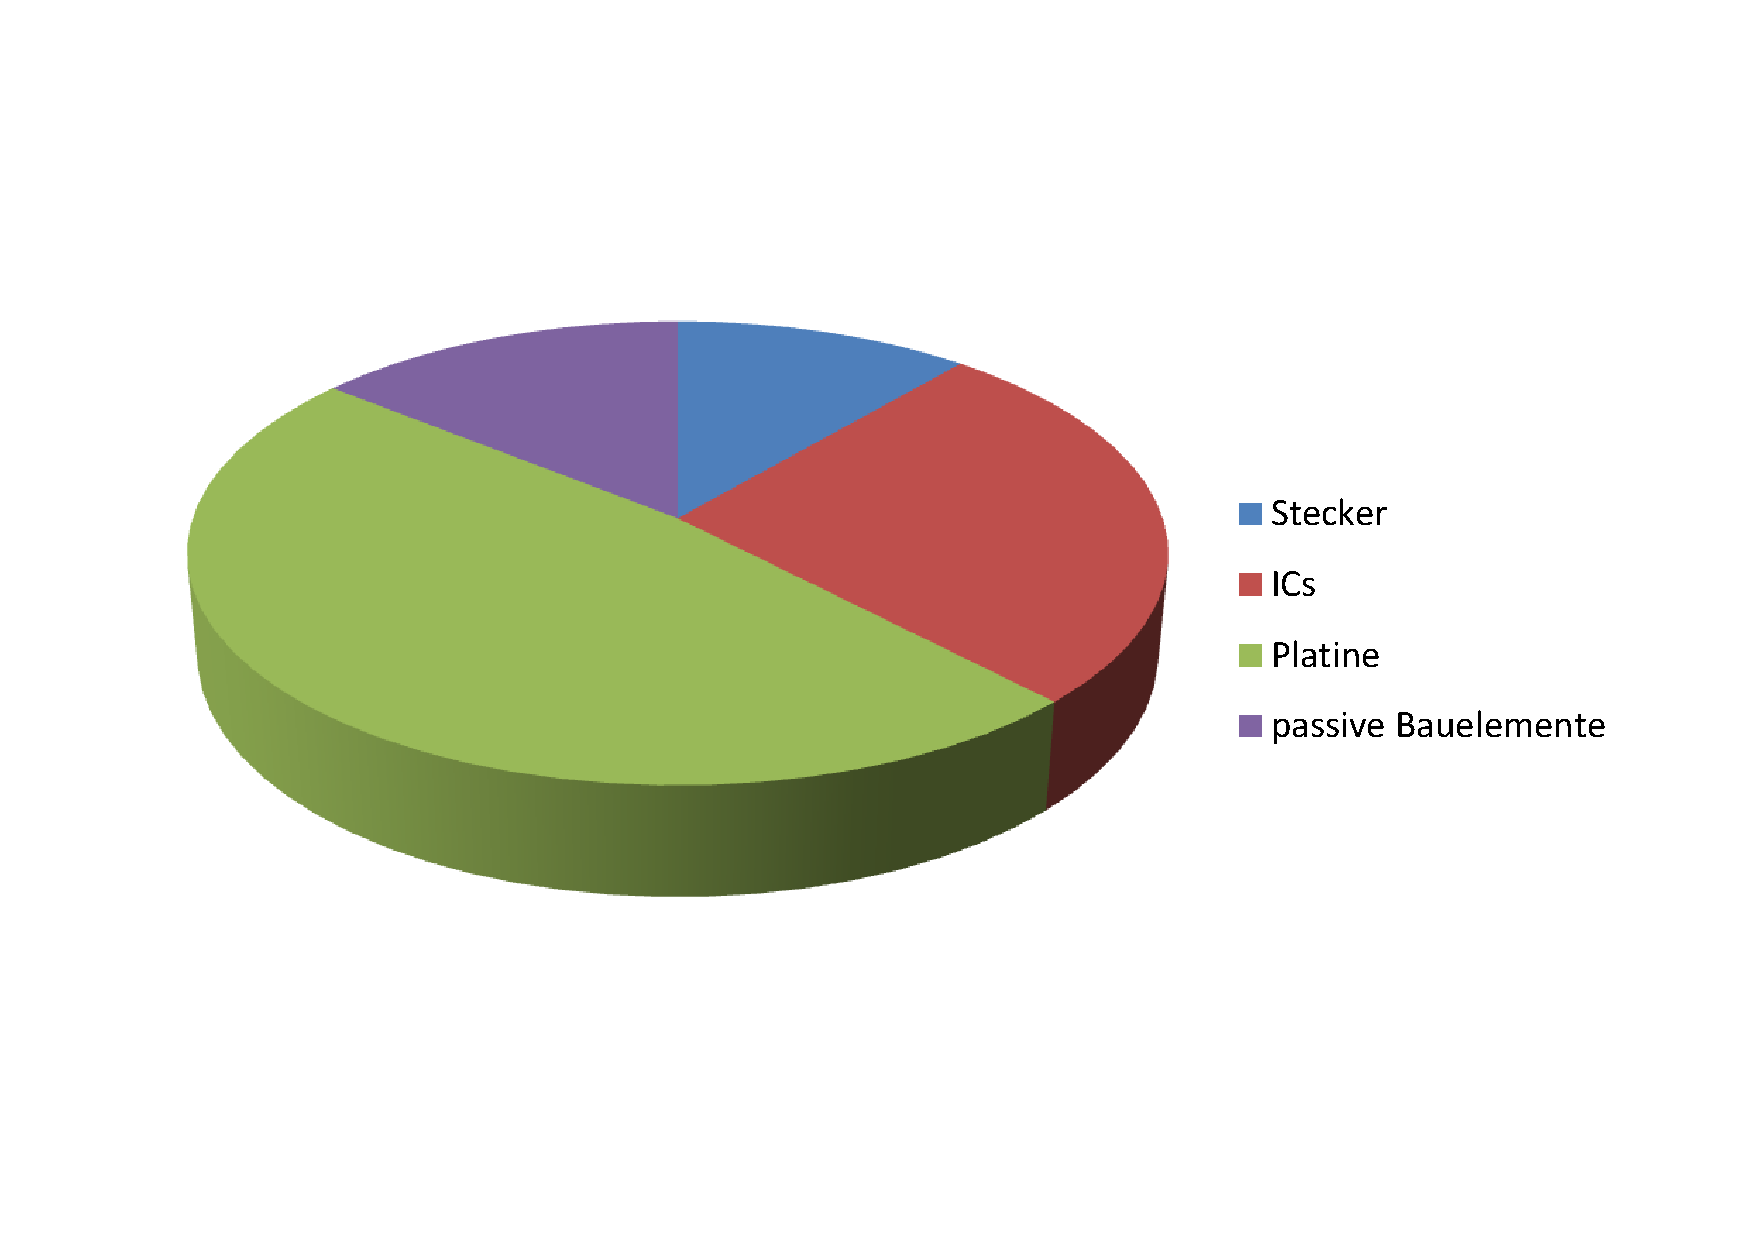
\includegraphics[width=\textwidth]{./Bilder/Platinenkosten.pdf}
\end{minipage}
\begin{minipage}[h]{0.5\textwidth}
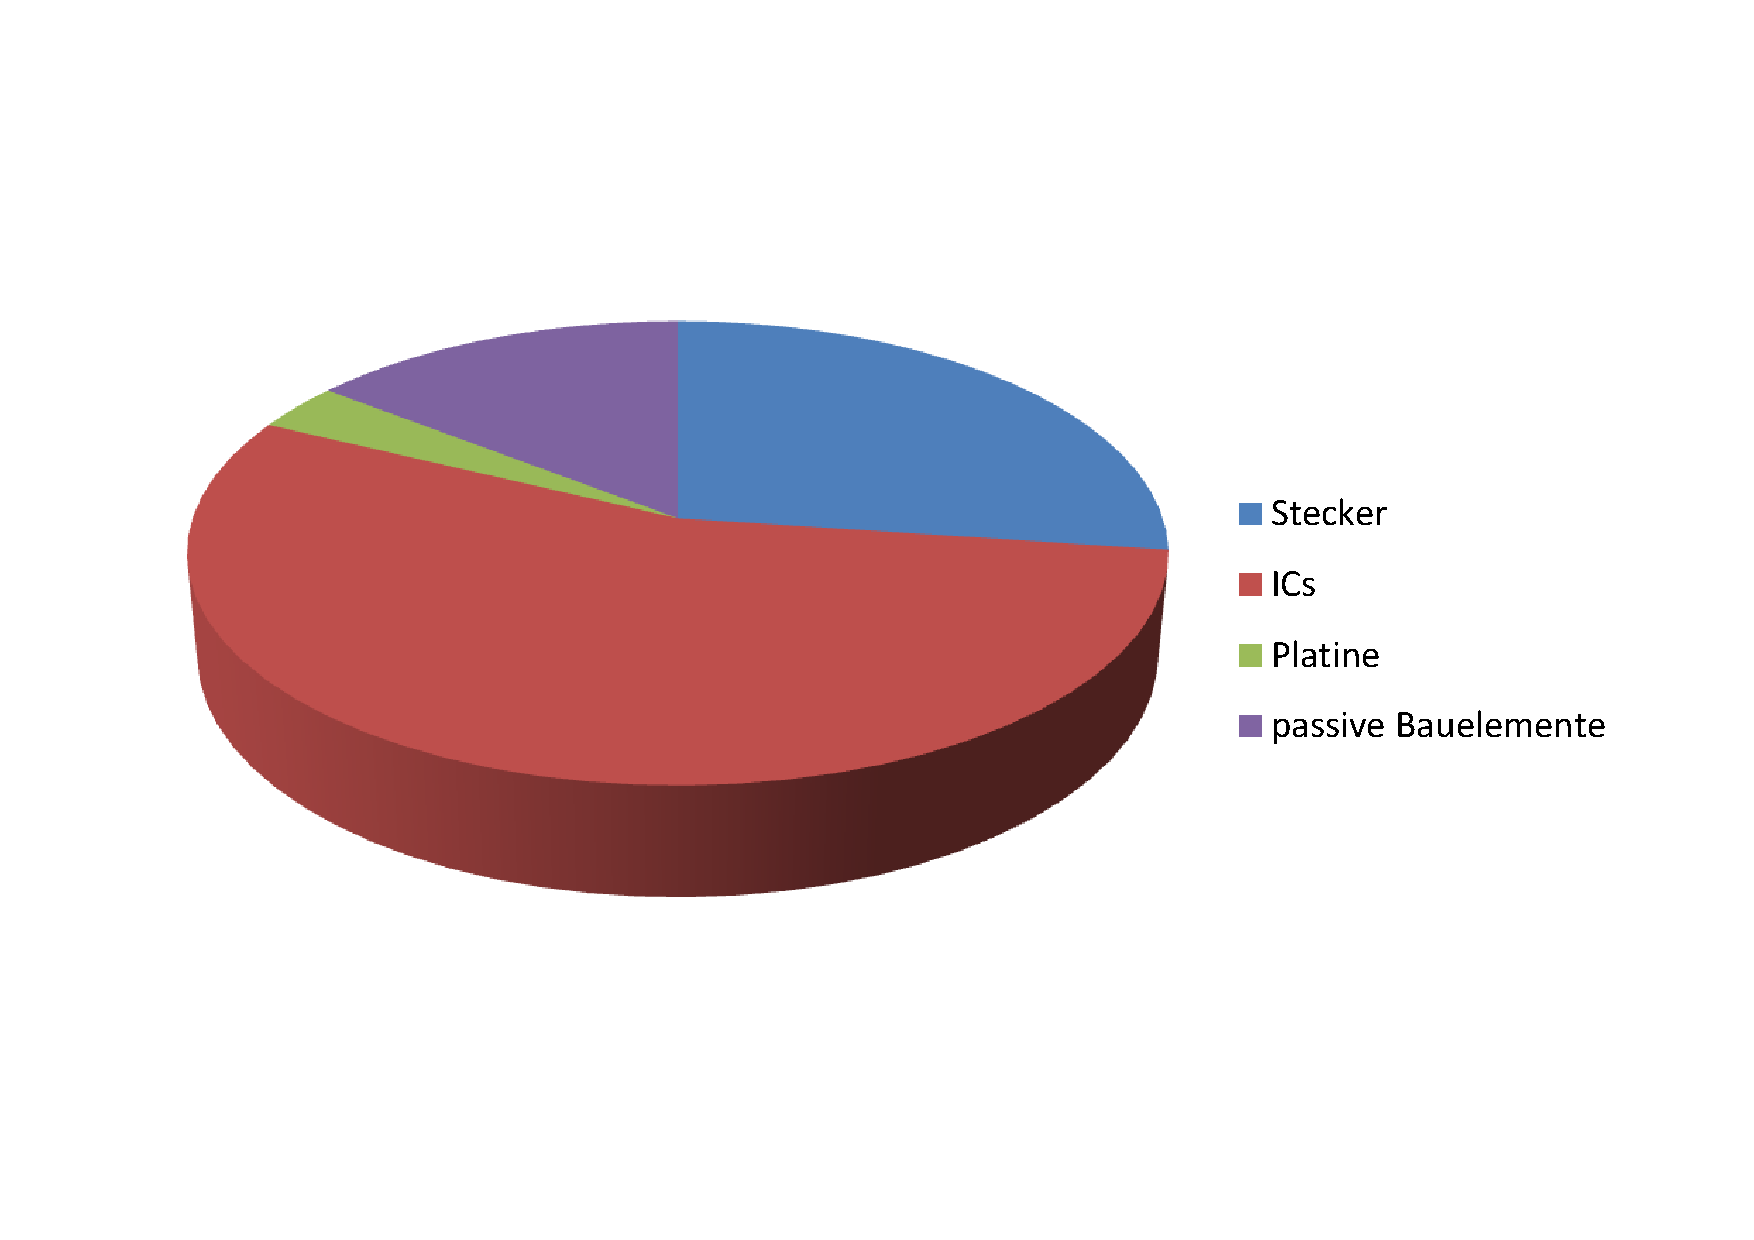
\includegraphics[width=\textwidth]{./Bilder/Platinenkosten-tausend.pdf}
\end{minipage}
\caption{Aufteilung der Kosten für die Stückzahlen 1 (links) und 1000 (rechts)}
	\label{fig:LDO}
\end{figure}

Es ist zu erkennen, dass die Platine bei geringen Stückzahlen ungefähr die Hälfte der Kosten ausmacht, während sie bei hohen Stückzahlen fast gar nicht mehr ins Gewicht fällt. Bei hohen Stückzahlen sind der größte Kostenfaktor die ICs. 
Ein Preisvergleich mit direkter Konkurrenz fällt schwer, da es wenig äquivalente Produkte auf dem Markt gibt, jedoch können die beiden vorherig am Prüfstand verwendeten Motortreiber zum Vergleich gezogen werden, die nur einen Teil der Platinenfunktionen abdecken. Der Kaufpreis des Motorcontrollers MDC1460 des Herstellers RoboteQ liegt bei circa 260 Euro (bei über vierfachem Bauraum), der Kaufpreis des Arduino IBT\_2 Motortreibers liegt bei circa 15 Euro. Zu bemerken ist, dass sich die Kosten der Platine auch mit einem mit einzurechnenden Gewinnaufschlag innerhalb des Preisrahmens der beiden Motortreiber bewegt, obwohl sie deutlich mehr Funktionen hat.

\section{Platinendesign-Analyse}\label{sec:platan}
Die Platine erfüllt für den derzeitigen Aktor die Aufgaben über Positionsregelung bei Schaltvorgängen, Überwachung der Umgebung (Temperatur, Eingangsspannung, Ausgangsstrom) und die Kommunikation mittels CAN-Nachrichten. Bisher sind keine bedeutsamen Probleme mit EMV aufgetreten, sodass die Sensorik auch bei Ansteuerung der Halbbrücken funktioniert und die CAN-Kommunikation erhalten bleibt. Die Anforderung an eine kompakte Baugröße wird mit 88,8x\SI{50}{mm} erfüllt. Eine einfache Handhabung in der Peripherie wird über den Anschlussstecker erreicht. Im Falle von Softwareupdates lässt sich der Betriebstecker leicht entfernen und die Updates über den Programmierstecker flashen, was in \autoref{sec:stecker} genauer behandelt wird. Sollten im Betrieb nach Einführen des neuen Aktors trotz der Schirmungsmaßnahmen Probleme mit EMV auftreten, so wird empfohlen das Platinendesign auf ein 4-Layer Design zu erweitern, um wie in \autoref{kap5} beschrieben, zusätzliche GND-Planes einfügen zu können. Weiterhin bleiben die LDOs der \SI{3,3}{V} und \SI{5}{V} Schiene zu beobachten, da diese beim Anschluss der Autobatterie relativ viel Wärme abgeben müssen um auf die jeweiligen Spannungsebenen zu regeln. Derzeit sind keine Probleme damit aufgetreten jedoch kann das Verhalten im Dauerbetrieb noch nicht vollständig abgeschätzt werden. Falls keine Probleme auftreten wird empfohlen diese auch bei Einführung eines 4-Layer Designs beizubehalten, da die LDOs konstante Spannungen ohne switching Charakteristiken liefern. Bei Problemen könnte ein Buck-Spannungsregler statt des \SI{5}{V} LDOs eingeführt werden, welcher von Batteriespannung auf die \SI{5}{V} regelt. Für die \SI{3}{V} könnte weiterhin ein LDO verwendet werden, welcher als VCC die \SI{5}{V} des Buck-Spannungsreglers nutzt. Damit wäre die Stabilität der \SI{3}{V} Versorgung für die ADC-Genauigkeit gesichert und das Problem entstehender Wärmeverluste reduziert. Allerdings könnte in dieser Verschaltung die Genauigkeit des Lagesensors nicht auf dem aktuellen Niveau garantiert werden, da dieser an die \SI{5}{V} angeschlossen ist und der Buck-Spannungsregler weniger konstante Spannungen ausgibt als ein LDO. 

\section{Regelergebnisse} \label{reglerergebnisse}
In \autoref{fig:shift_gear2} und \autoref{fig:shift_toneutral} sind die exemplarisch gemessenen Positionsverläufe, Regelabweichungen und Stellgrößen für das Schalten von Gang 2 zu Neutral und umgekehrt aufgetragen. Das Schalten von und nach Gang 1 wird nicht betrachtet, da der verbaute Synchronring die Regelung bei einer Drehzahl $n=0$ zu stark behindert.\\
Die Messungen wurden hinreichend oft durchgeführt, sodass eine Reproduzierbarkeit der Ergebnisse sichergestellt werden konnte. Die Sollwerte sind jeweils mit roten Linien gekennzeichnet und betragen für den zweiten Gang \SI{10}{mm} und Neutral \SI{0}{mm}. Für beide wurde ein Toleranzband festgelegt, dass \SI{10}{\%} der Sprunghöhe zwischen den Gängen entspricht. Der verwendete PID-Regler mit Störgrößenkompensation wurde in \autoref{regler} beschrieben.

\subsection{Schalten in Gang 2}

Für das Schalten in Gang 2 ist in \autoref{fig:shift_gear2} ein Überschwingen von \SI{380}{\mu m} zu beobachten. Dies kann allerdings auf die lose Befestigung des Lagesensors im Prüfstand zurückgeführt werden. Der Schaltvorgang bringt den ganzen Prüfstand kurzzeitig zum Schwingen, sodass der Lagesensor eine zusätzliche relative Bewegung zur Läuferstange erfährt. Die Sollposition wird erstmals nach \SI{36}{ms} erreicht und verlässt das Toleranzband nach einer Dauer von \SI{54}{ms} nicht mehr. In dem Verlauf der Stellgröße zeigt sich, dass für den Schaltvorgang das maximale PWM-Signal bei \SI{63}{\%} liegt und somit ein großer Anteil der möglichen Stromdurchschaltung gar nicht ausgenutzt wird. Die Stellgröße bleibt nahezu konstant, bis ca. \SI{2}{mm} vor dem Erreichen der Sollposition. Anschließend fällt sie kurzzeitig ins Negative, bevor sie bei \SI{0}{\%} einpendelt.  

\subsection{Schalten in Neutral}
Bei diesem Schaltvorgang zeigt \autoref{fig:shift_toneutral} ein erstes Überschwingen von \SI{288}{\mu m} über den Sollwert. Auch dieses Überschwingen kann durch die Bewegung des Sensors erklärt werden. Die Sollwertvorgabe wird nach \SI{39}{ms} zum ersten Mal erreicht und dessen Toleranzband wird nach \SI{50}{ms} nicht mehr verlassen. Die Stellgröße springt zu Beginn des Schaltvorgangs auf ein PWM-Signal von \SI{-72}{\%}, was anschließend betragsmäßig bis zu einer Regelabweichung von\SI{1,4}{mm}auf einen Wert von \SI{-28}{\%} abnimmt. An dieser Stelle springt das PWM-Signal in den niedrigen positiven Bereich, bevor es bei \SI{0}{\%} einpendelt.

\subsection{Diskussion der Regelergebnisse}\label{diskreg}
Die beiden Schaltvorgänge erreichen ihren Sollwert und die zugehörige stationäre Genauigkeit in unter \SI{50}{ms}, was die Anforderungen von einer Schaltzeit \SI{\leq100}{ms} klar erfüllt. Für die stationäre Genauigkeit ist die korrekte Positionierung des Lagesensors von entscheidender Bedeutung. Diese Postion bleibt allerdings nicht über alle Schalttvorgänge gleich, aufgrund der losen Halterung und den Erschütterungen des Prüfstands. Abhilfe könnte hier eine besserer Fixierung schaffen, wodurch die Regelergebnisse weiter verbessert werden könnten. Aber auch unter Annahme, dass die Überschwingungen nicht auf den Lagesensor zurückzuführen sind, stellen sie aufgrund ihrer geringen Größe (\SI{\leq400}{\mu m}) kein Problem dar. Erst ab einem Überschwingen von \SI{\geq1}{mm} wäre in der Neutralstellung die Gefahr des unabsichtlichen Schaltens in einen anderen Gang gegeben.\\
In den Verläufen der Stellgrößen ist zu erkennen, dass der Aktor ab ca. \SI{1-2}{mm} nicht mehr beschleunigt, sondern leicht abgebremst wird.\\
Mit der erreichten stationären Genauigkeit sind die Bedingungen für eine erfolgreiche Implementierung eines Haltereglers erfüllt. Dabei wird der Positionsregler durch einen anderen Regler abgelöst, sobald die Position das Toleranzband für eine bestimme Zeit nicht mehr verlässt. Die Aufgabe des neuen Reglers besteht dann lediglich darin die Postion zu halten, bis ein neuer Schaltbefehl erfolgt. Hauptproblem für diesen Regler ist der Haftgleiteffekt, welcher auf der Tatsache beruht, dass der Haftreibungskoeffizient größer als der Gleitreibungskoeffizient ist \cite{Bowden2001}. 

\begin{figure} [H]
	\centering
	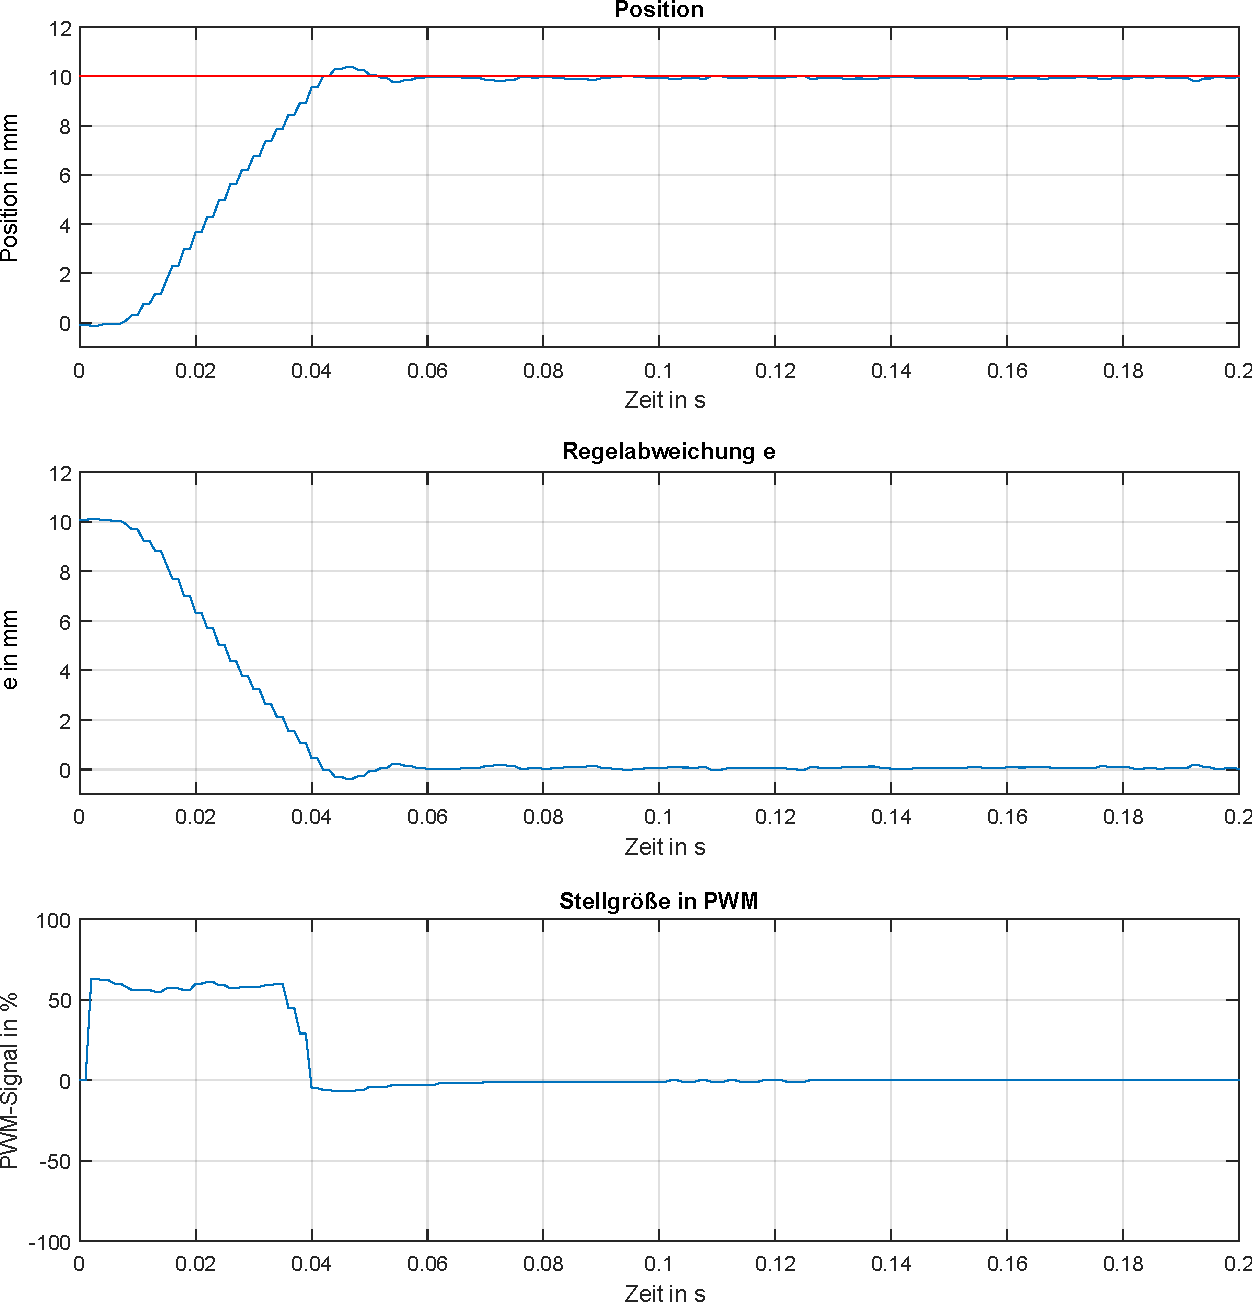
\includegraphics[width=1\columnwidth]{Bilder/shift_gear2_test.pdf}
	\caption{Position, Regelabweichung und Stellgröße für das Schalten in Gang 2}
	\label{fig:shift_gear2}
\end{figure}

\begin{figure} [H]
	\centering
	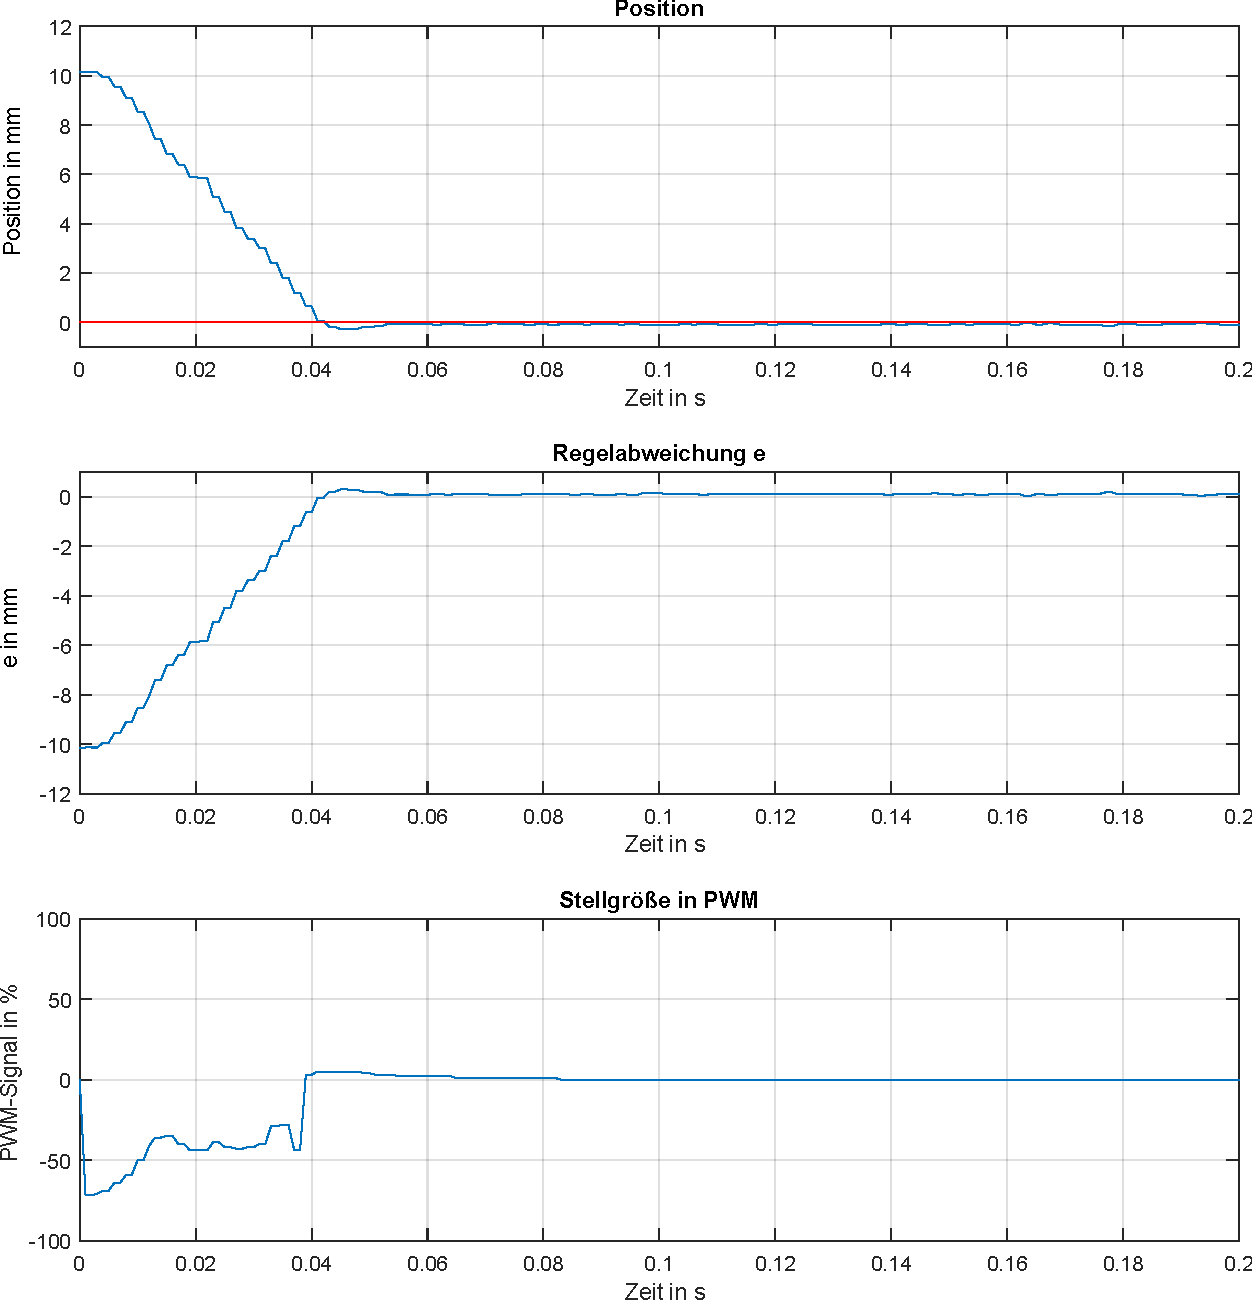
\includegraphics[width=1\linewidth]{Bilder/shift_toneutral.pdf}
	\caption{Position, Regelabweichung und Stellgröße für das Schalten in Neutral}
	\label{fig:shift_toneutral}
\end{figure}

\subsection{Schaltgabelkraft am Anschlag}\label{schaltgabelkraft}
In \autoref{fig:aktor_anschlag} ist ein Schaltvorgang von Neutral in Gang 2 und die zugehörige Strommessung des Aktors aufgetragen. Zu sehen ist, dass beim Erreichen der Sollgröße zum Zeitpunkt $t$ = \SI{0,1316}{s} nur etwa \SI{0,1}{A} im Aktor fließt. Das bedeutet, dass die Lorentzkraft der Spule auf den Läufer gemäß \autoref{eq:lorentz} keine nennenswerte Kraft auf den Aktor ausübt. Somit wirkt auf den Läufer zu diesem Zeitpunkt fast ausschließlich die Kraft aufgrund seiner Massenträgheit. Nach dem Übertreten des Läufers der Sollposition reagiert die Regelung durch Gegenbestromung, sodass die Massenträgheit durch die Lorentzkraft gehemmt wird und der Läufer in Richtung Sollposition gebracht wird. Die Anschlagskraft wird somit minimiert.

\begin{figure} [h]
	\centering
	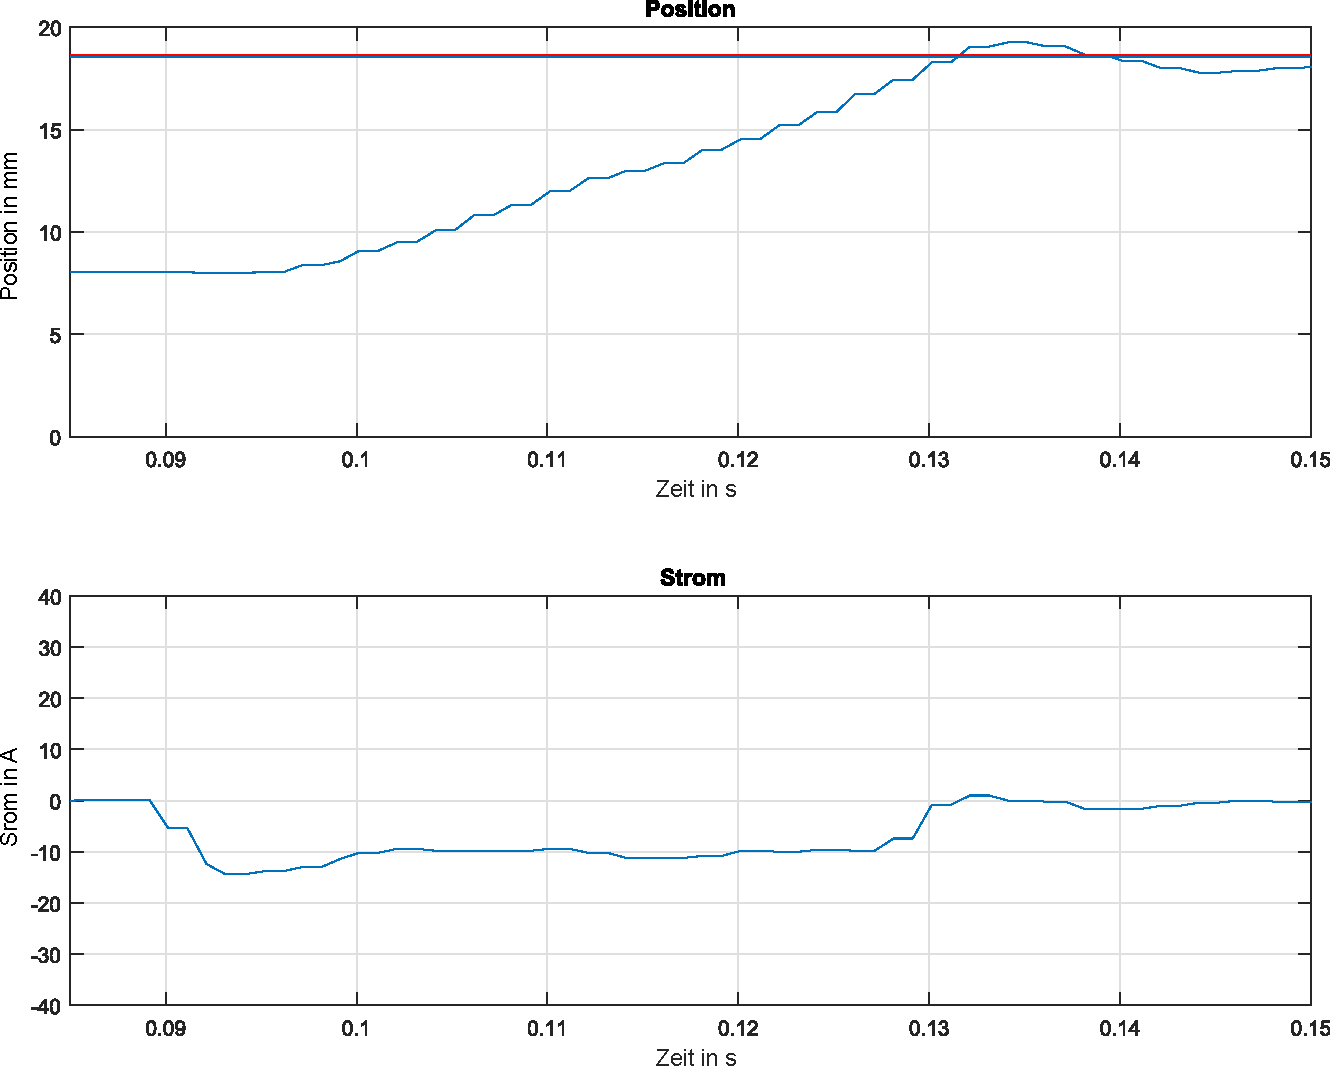
\includegraphics[width=1\linewidth]{Bilder/aktor_anschlag2}
	\caption{Strommessung im Schaltvorgang von Neutral in Gang 2}
	\label{fig:aktor_anschlag}
\end{figure}